\documentclass{standalone}

\usepackage{tikz}
\usepackage{circuitikz}


         
\begin{document}
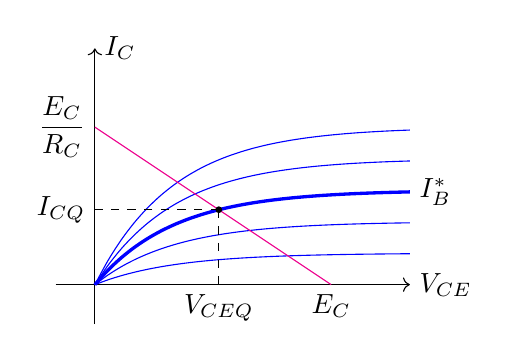
\begin{tikzpicture}[scale=2]
    \draw[->](-0.25,0)--(2,0)node[right]{$V_{CE}$};
    \draw[->](0,-0.25)--(0,1.5)node[right]{$I_C$};

    \draw[blue, smooth, domain=0:2]plot (\x,{0.2*(1-e^(-2*\x))});
    \draw[blue, smooth, domain=0:2]plot (\x,{0.4*(1-e^(-2*\x))});
    \draw[very thick,blue, smooth, domain=0:2]plot (\x,{0.6*(1-e^(-2*\x))});
    \draw[blue, smooth, domain=0:2]plot (\x,{0.8*(1-e^(-2*\x))});
    \draw[blue, smooth, domain=0:2]plot (\x,{(1-e^(-2*\x))});

    \draw[magenta] (0,1)node[left,black]{$\displaystyle\frac{E_C}{R_C}$}--(1.5,0)node[below,black]{$E_C$};
    \node[right]at(2,0.589){$I_B^*$};
    \filldraw[black](0.787,0.476)circle(0.5pt);
    \draw[dashed](0.787,0.476)--(0,0.476)node[left]{$I_{CQ}$};
    \draw[dashed](0.787,0.476)--(0.787,0)node[below]{$V_{CEQ}$};
\end{tikzpicture}
\end{document}